So far, only 2D monoblocks simulations were run, assuming an infinite thickness (or assuming no desorption from the poloidal gaps).
The goal of this section is to assess the influence of 3D edge effects on the monoblocks simulation results.
It will be shown that the error induced by 2D assumption decreases for thick monoblocks.

\subsection{Methodology}

The DEMO monoblock geometry differs slightly from the ITER geometry (see Figure \ref{fig: geometry DEMO monoblock}) but the general concept is the same, meaning the observations made in this Section are also valid for the ITER geometry.


\begin{figure}
    \centering
        \begin{overpic}[width=\linewidth]{Figures/Chapter3/monoblocks/3D_monoblocks/sketch.pdf}
            \put(21, 15){\SI{23}{mm}}
            \put(51, 50){\SI{25}{mm}}
            % \put(21, 15){\SI{13.5}{mm}}
            \put(21, 56){ \diameter \SI{12}{mm}}
            \put(21, 63){ \diameter \SI{15}{mm}}
            \put(21, 68){ \diameter \SI{17}{mm}}
            \put(10, 70){\large$\Gamma_\mathrm{top}$}
            \put(0, 60){\large$\Gamma_\mathrm{toroidal}$}
            \put(43, 60){\large$\Gamma_\mathrm{toroidal}$}
            \put(21, 45){\large$\Gamma_\mathrm{coolant}$}
            \put(68, 71){e}
            \put(66, 50){e + \SI{1}{mm}}
            \put(60, 60){\large$\Gamma_\mathrm{poloidal}$}
            \put(75, 60){\large$\Gamma_\mathrm{poloidal}$}
        \end{overpic}
    \caption{3D geometry of the DEMO monoblock used for the simulations showing W armour \cruleme[grey]{0.3cm}{0.3cm}, Cu interlayer \cruleme[orange]{0.3cm}{0.3cm}, CuCrZr alloy cooling pipe  \cruleme[yellow]{0.3cm}{0.3cm}.}
    \label{fig: geometry DEMO monoblock}
\end{figure}

The boundary conditions for the steady state heat transfer problem are the same as for the 2D case (see Equation \ref{eq: bc thermal DEMO monoblock}).
The boundary conditions for the transient H transport problem are similar (see Equations \ref{eq: bc H transport DEMO monoblock}).
A non-homogeneous mobile concentration is assumed at the plasma exposed surface to simulate an implanted source of particles (see Section \ref{triangle model}).
Depending on the simulation case (with or without desorption on the gaps), the other external surfaces (except the cooling surfaces) will either be insulated or an instantaneous recombination will be assumed.


\begin{subequations}
    \begin{align}
    -\lambda \vec{\nabla} T \cdot \vec{n} &=\varphi_\mathrm{heat} \quad  &\text { on } \Gamma_\mathrm{top}\\
    -\lambda \vec{\nabla} T\cdot \vec{n} &= -h \cdot \left(T_\mathrm{coolant} - T\right)\quad &\text { on } \Gamma_\mathrm{coolant}
    \end{align}
    \label{eq: bc thermal DEMO monoblock}
\end{subequations}
where $\varphi_\mathrm{heat}=\SI{10}{MW}$, $h=\SI{7e4}{W.m^{-2}.K^{-1}}$ is the heat exchange coefficient and $T_\mathrm{coolant} = \SI{323}{K}$ is the coolant temperature.

\begin{subequations}
    \begin{align}
    c_\mathrm{m} &=  \frac{\varphi_\mathrm{imp} R_p}{D} \quad &\text { on } \Gamma_\mathrm{top}\\
    -D \vec{\nabla} c_\mathrm{m} \cdot \vec{n} &= K_\mathrm{CuCrZr} \cdot c_\mathrm{m}^{2} \quad &\text { on } \Gamma_\mathrm{coolant} \\
    c_\mathrm{m} &=  0 \quad &\text { on } \Gamma_\mathrm{toroidal} \text{  and  } \Gamma_\mathrm{pipe} \\
    c_\mathrm{m} &=  0 \quad \text{or} \quad -D \vec{\nabla} c_\mathrm{m} \cdot \vec{n} = 0 &\text { on } \Gamma_\mathrm{poloidal}
    \end{align}
    \label{eq: bc H transport DEMO monoblock}
\end{subequations}
where $\varphi_\mathrm{imp} = \SI{1.6e22}{H.m^{-2}.s^{-1}}$ is the implanted particle flux, $R_p = \SI{1e-9}{m}$ is the particle implantation depth, $K_\mathrm{CuCrZr}=2.9\times 10^{-14}\exp{-1.92/(k_B T)}$ is the H recombination coefficient in CuCrZr expressed in \si{m^4.s^{-1}}.

Two intrinsic traps were set in W, one trap in the Cu interlayer and two traps in the CuCrZr cooling pipe (see Table \ref{tab:traps monoblock DEMO}).

\begin{table*}
    \centering
    \begin{tabular}{L{1.5cm} L{1.5cm} R{1.6cm} R{1.1cm} R{1.6cm} R{1.1cm} R{2cm}}
         & Material & $k_0 (\si{m^3.s^{-1}})$ &  $E_k (\si{eV})$ & $p_0 (\si{s^{-1}})$ & $E_p (\si{eV})$ & $n_i (\si{at.fr.})$ \\
        \hline
        \\
        Trap 1 & W & $8.96 \times 10^{-17}$ & 0.39 & $1 \times 10^{13}$& 0.87 & $1.0 \times 10^{-3}$ \\
        \\
        Trap 2 & W & $8.96 \times 10^{-17}$ & 0.39 & $1 \times 10^{13}$& 1.00 & $4.0 \times 10^{-4}$ \\
        \\
        Trap 3 & Cu & $6.0 \times 10^{-17}$ & 0.39 & $8.0 \times 10^{13}$ & 0.50 &$5.0 \times 10^{-5}$\\
        \\
        Trap 4 & CuCrZr & $1.2\times 10^{-16}$ & 0.42 & $8.0 \times 10^{13}$ & 0.85 &$5.0 \times 10^{-5}$\\
        \\
        % Trap 5 & CuCrZr & $1.2\times 10^{-16}$ & 0.42 & $8.0 \times 10^{13}$ & 0.83 &$4.0 \times 10^{-2}$\\
        % \\
    \end{tabular}
    \caption{Traps properties used in the 3D DEMO monoblocks simulations.}
    \label{tab:traps monoblock DEMO}
\end{table*}

Transient simulations up to \SI{e7}{s} were run.

\subsection{Standard case}

FESTIM simulations were run with and without desorption on the gaps.

% Temperature field

The temperature field obtained was very similar to the 2D case (see Figure \ref{fig: T field 3D monoblock}) with a top surface temperature of approximately \SI{1200}{K}.

\begin{figure} [h]
    \centering
    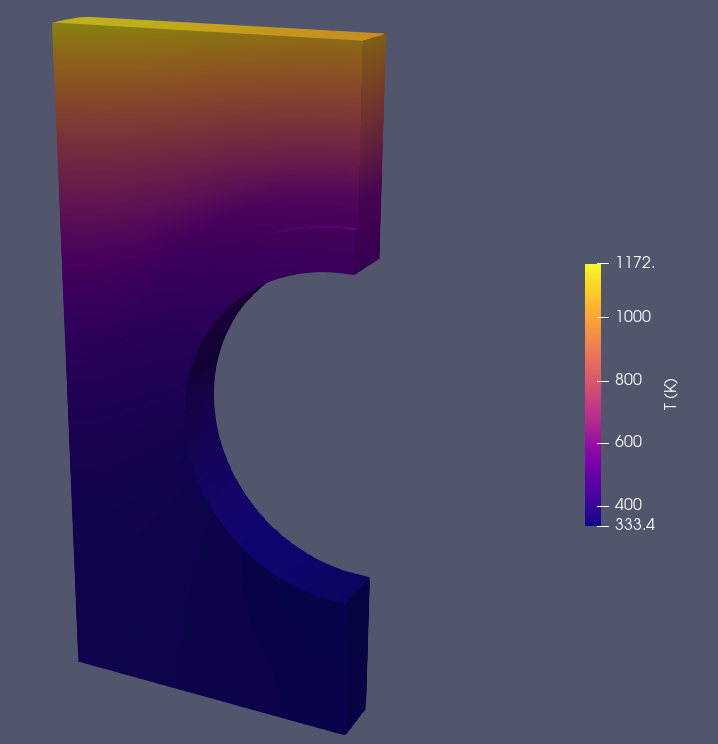
\includegraphics[width=\linewidth]{Figures/Chapter3/monoblocks/3D_monoblocks/temperature_3D_monoblock.png}
    \caption{Temperature field of the 3D DEMO monoblock.}
    \label{fig: T field 3D monoblock}
\end{figure}


% Retention fields
As expected, a higher retention was observed in the case without desorption (see Figure \ref{fig:retention fields 3D monoblocks}).
This is explained by the surface losses.
% The maximum retention for the case with desorption is three orders of magnitude lower than that of the case without desorption.
% In both cases, the higher retention was found to be in the CuCrZr cooling pipe.
% This is consistent with the obsverations made previously.

\begin{figure} [h]
    \centering
    \begin{subfigure}{0.45\linewidth}
        \centering
        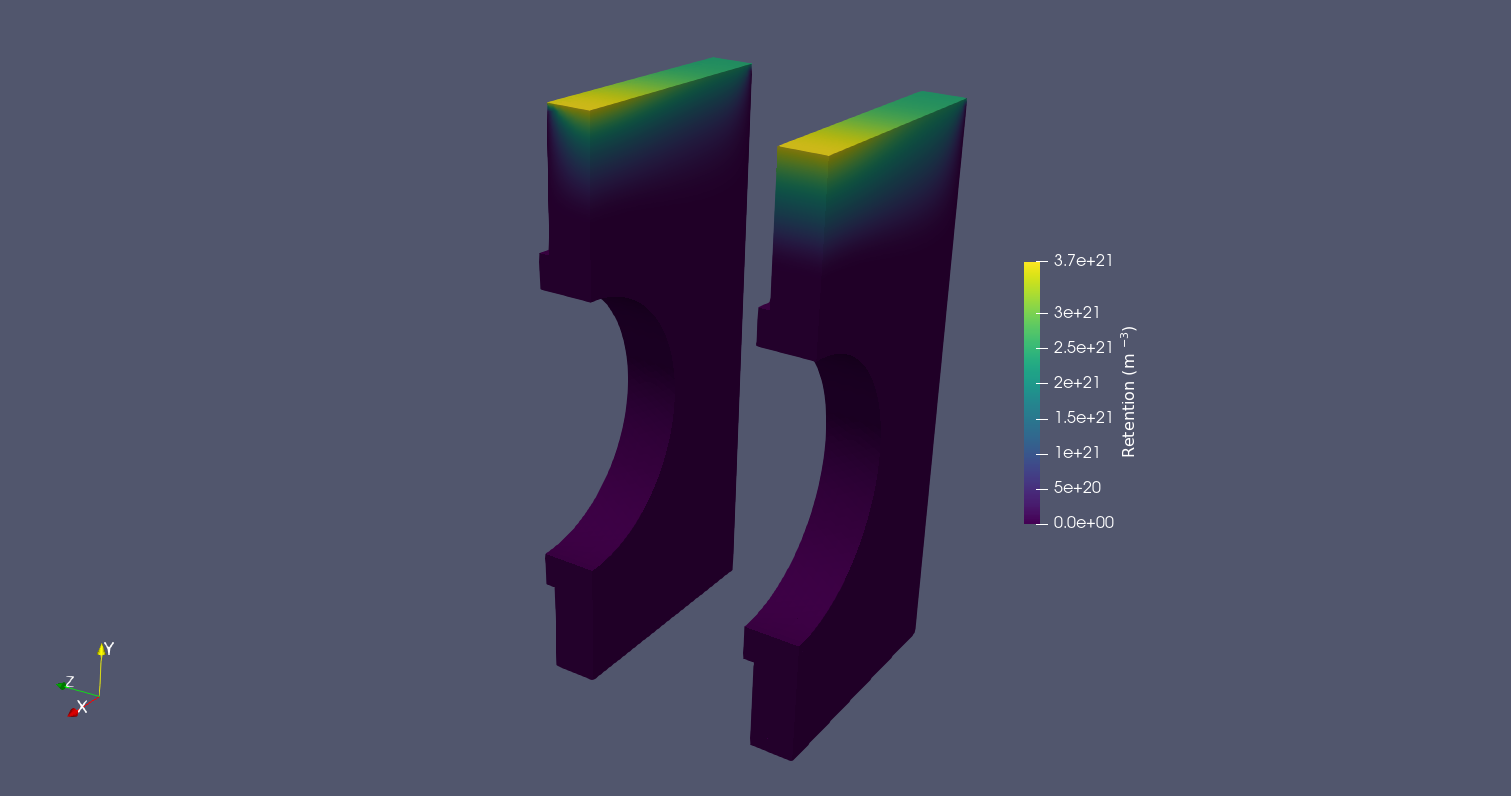
\includegraphics[trim=500 0 300 0, clip, width=\linewidth]{Figures/Chapter3/monoblocks/3D_monoblocks/retention_1e3s.png}
        \caption{$t=\SI{1e3}{s}$}
    \end{subfigure}%
    \qquad
    \begin{subfigure}{0.45\linewidth}
        \centering
        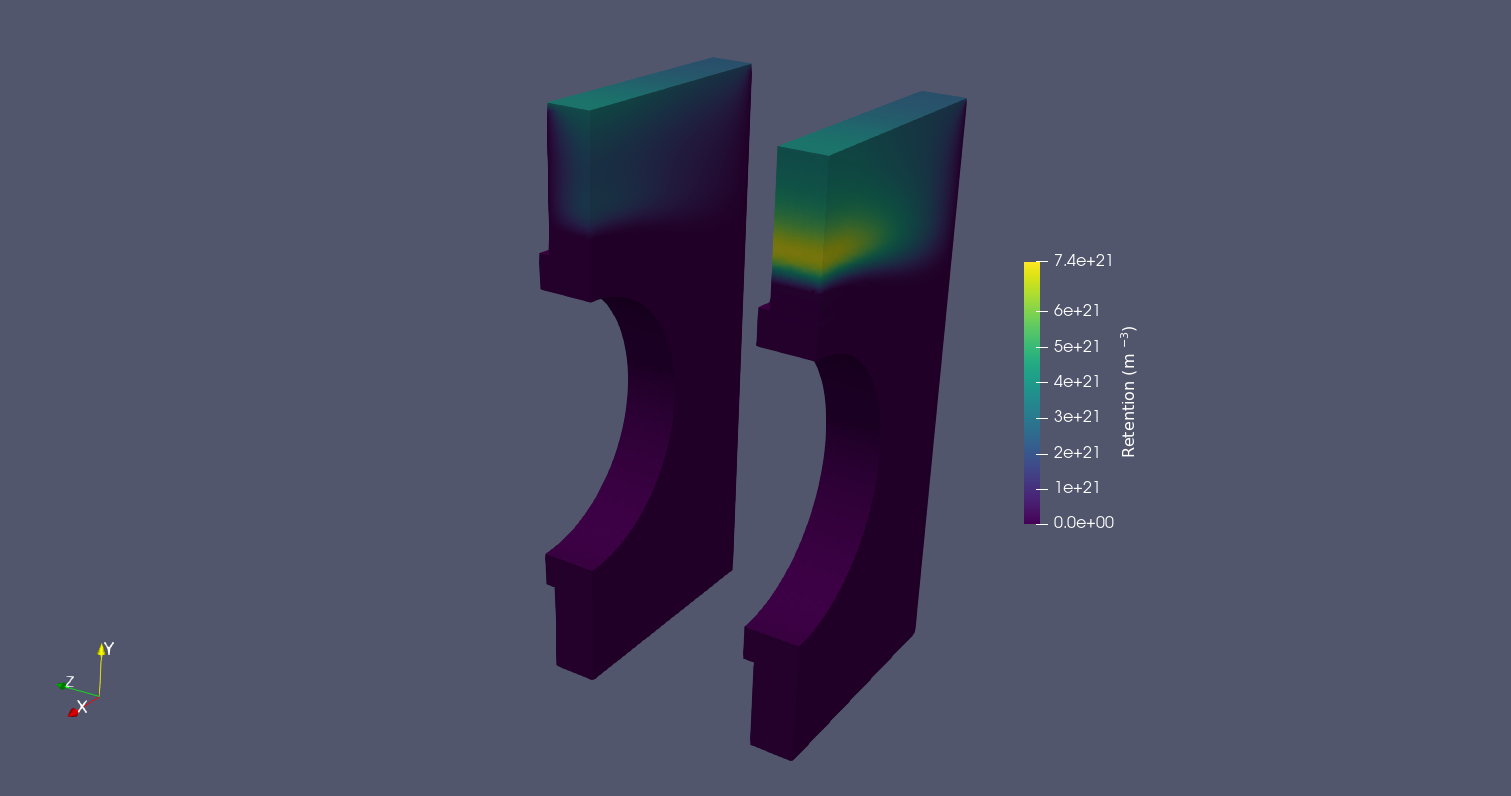
\includegraphics[trim=500 0 300 0, clip, width=\linewidth]{Figures/Chapter3/monoblocks/3D_monoblocks/retention_1e4s.png}
        \caption{$t=\SI{1e4}{s}$}
    \end{subfigure}
    \begin{subfigure}{0.45\linewidth}
        \centering
        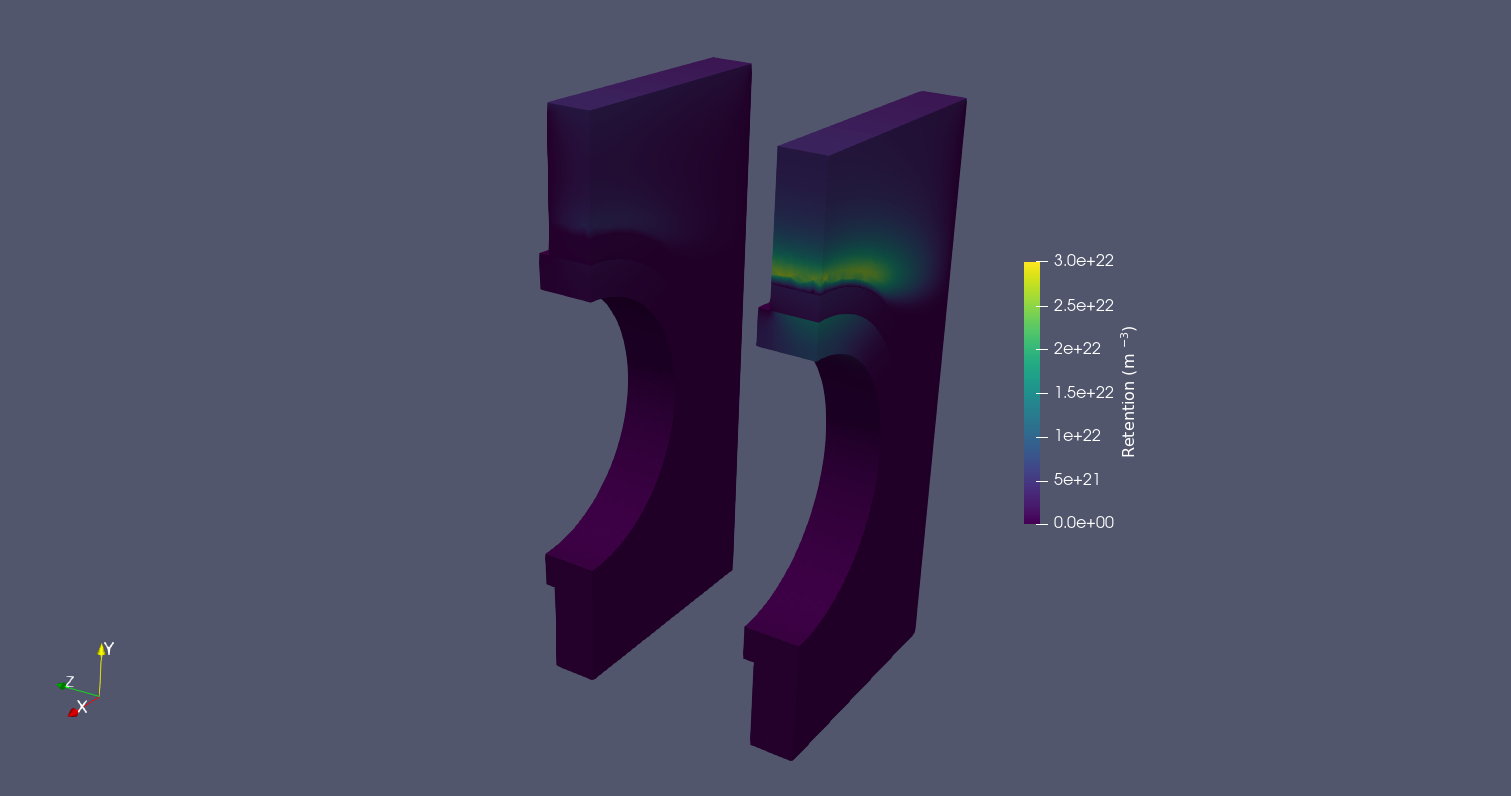
\includegraphics[trim=500 0 300 0, clip, width=\linewidth]{Figures/Chapter3/monoblocks/3D_monoblocks/retention_1e5s.png}
        \caption{$t=\SI{1e5}{s}$}
    \end{subfigure}%
    \qquad
    \begin{subfigure}{0.45\linewidth}
        \centering
        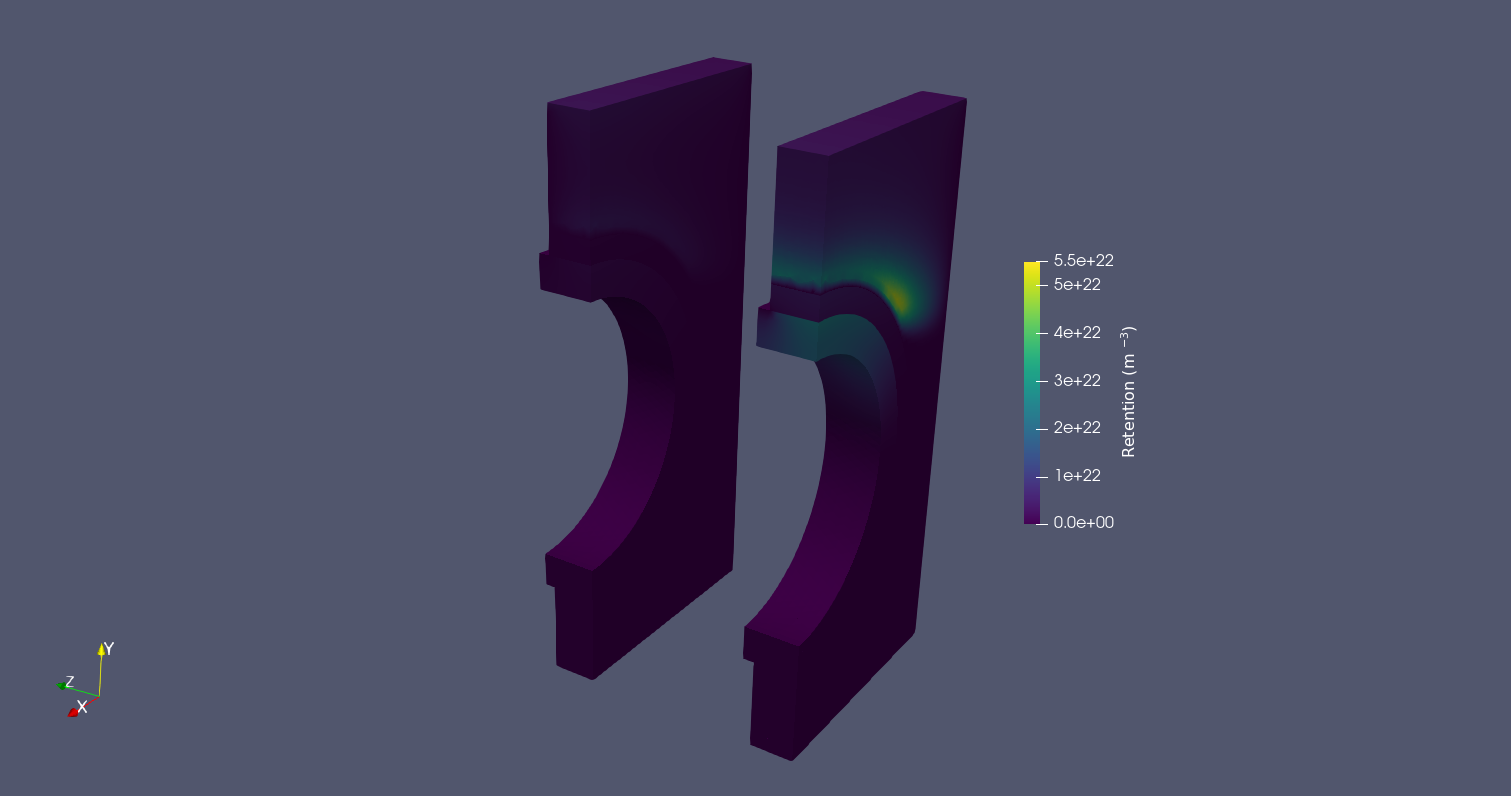
\includegraphics[trim=500 0 300 0, clip, width=\linewidth]{Figures/Chapter3/monoblocks/3D_monoblocks/retention_1e6s.png}
        \caption{$t=\SI{1e6}{s}$}
    \end{subfigure}
    \caption{Retention fields of the DEMO monoblock with (left) or without (right) recombination on the poloidal gaps (standard case). Note the colour bars are different.}
    \label{fig:retention fields 3D monoblocks}
\end{figure}

% Inventory
The total H inventory in the monoblock was also between one and three orders of magnitude lower in the case with desorption (see Figure \ref{fig: inventory vs time DEMO monoblock}).
This difference increased with the exposure time.
Moreover, the steady state was reached way earlier for the case with desorption whereas the inventory kept increasing after \SI{e7}{s} for the insulated case.
This means that not taking desorption from the gaps into account in 2D simulations is a conservative assumption in terms of H inventory.
The simulations performed in Section \ref{influence of exposure conditions} then overestimate the monoblock H inventory.

\begin{figure} [h]
    \centering
    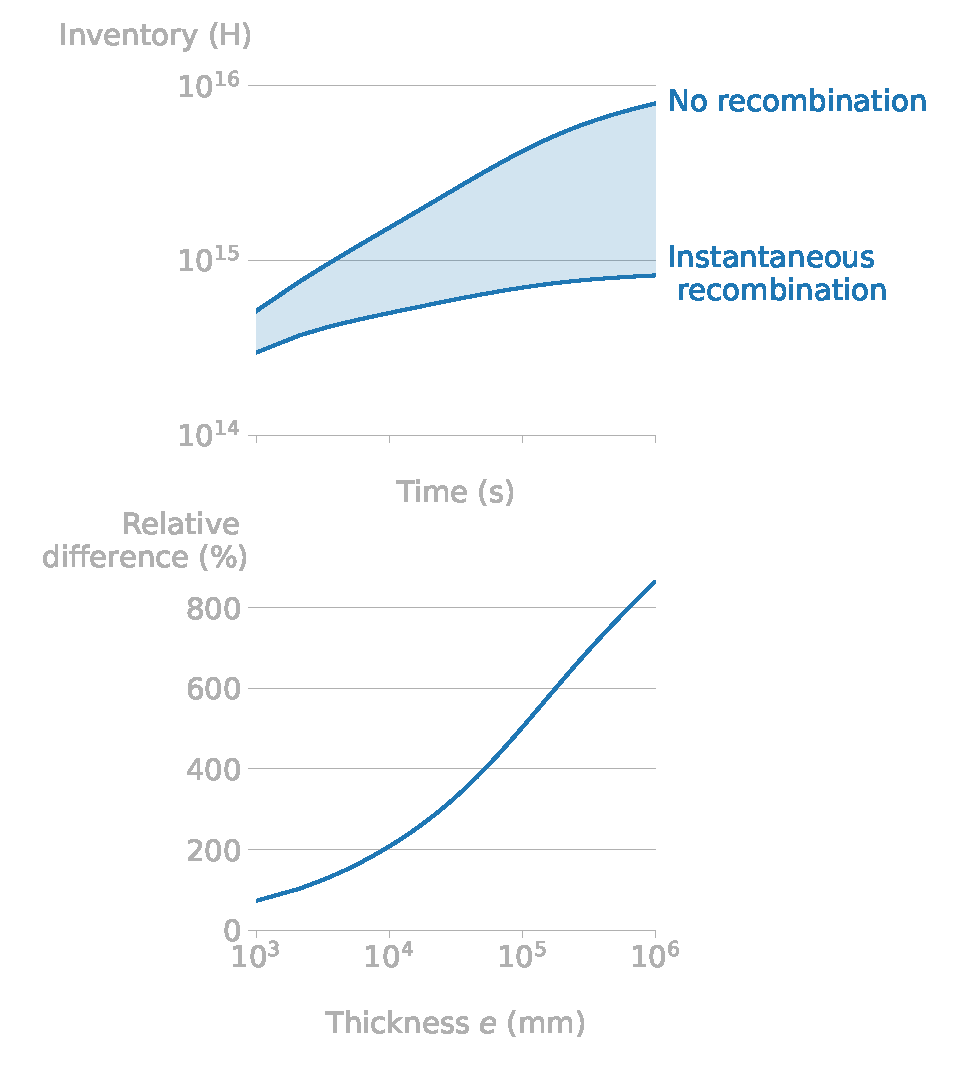
\includegraphics[width=\linewidth]{Figures/Chapter3/monoblocks/3D_monoblocks/inventory_standard_case_w_wo_recomb.pdf}
    \caption{Temporal evolution of the monoblock inventory (standard case).}
    \label{fig: inventory vs time DEMO monoblock}
\end{figure}

% fluxes
These 3D simulations are however essential to estimate the outgassing fluxes from the poloidal gaps.
The particle flux at the poloidal gap is six times higher than the flux at the toroidal gap  (see Figure \ref{fig: fluxes DEMO monoblock}).
The permeation flux to the coolant is five to six orders orders of magnitude lower than the fluxes at the gaps.
The particle fluxes at the gaps (poloidal and toroidal) were approximately \SI{e12}{H.s^{-1}} whereas the flux towards the cooling channel was below \SI{e7}{H.s^{-1}}.
The values of the outgassing fluxes from both the gaps are orders of magnitude lower than that of the retrodesorbed flux (\textit{ie} the flux of implanted particles that diffuse back to the exposed surface).
This means 3D edge effects will not affect previous results regarding the outgassing to the vessel.
They will however impact the value of the contamination flux towards the coolant as assuming an instantaneous recombination on the gaps will lead to way less particles reaching the cooling surface and therefore a lower flux.

\begin{figure} [h]
    \centering
    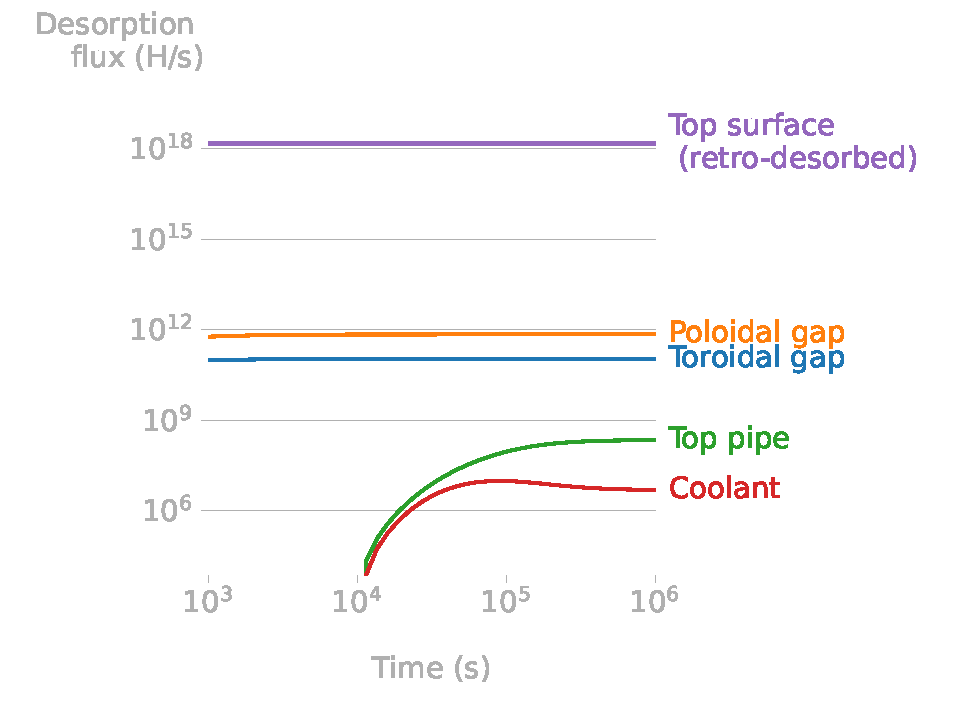
\includegraphics[width=\linewidth]{Figures/Chapter3/monoblocks/3D_monoblocks/desorption_flux_standard_case.pdf}
    \caption{Temporal evolution of outgassing fluxes for the standard case with desorption from the poloidal gaps. Blue lines correspond to the fluxes towards the vacuum vessel, the orange line is the flux towards the coolant.}
    \label{fig: fluxes DEMO monoblock}
\end{figure}

\subsection{Influence of the monoblock thickness}

Several simulations were run with monoblock thicknesses varying from \SI{4}{mm} to \SI{14}{mm}.

% inventory
As the thickness increases, the inventory per unit thickness increases for the case with instantaneous recombination on the poloidal gap (see Figure \ref{fig: inventory vs time DEMO monoblock}).
It remains constant for the case with no recombination since it is equivalent to a 2D case (the decrease observed at low thicknesses is due to the impact of the CuCrZr pipe between monoblocks as shown on Figure \ref{fig: geometry DEMO monoblock}).
The relative difference between the cases with or without recombination on the poloidal gap decreases as the thickness increases.
After \SI{1e6}{s} of exposure, for a thickness of \SI{4}{mm} the relative difference is \SI{200}{\%} and drops at \SI{30}{\%} for \SI{14}{mm}.
This result was expected as the edge effects become negligible at large thicknesses.

\begin{figure} [h]
    \centering
    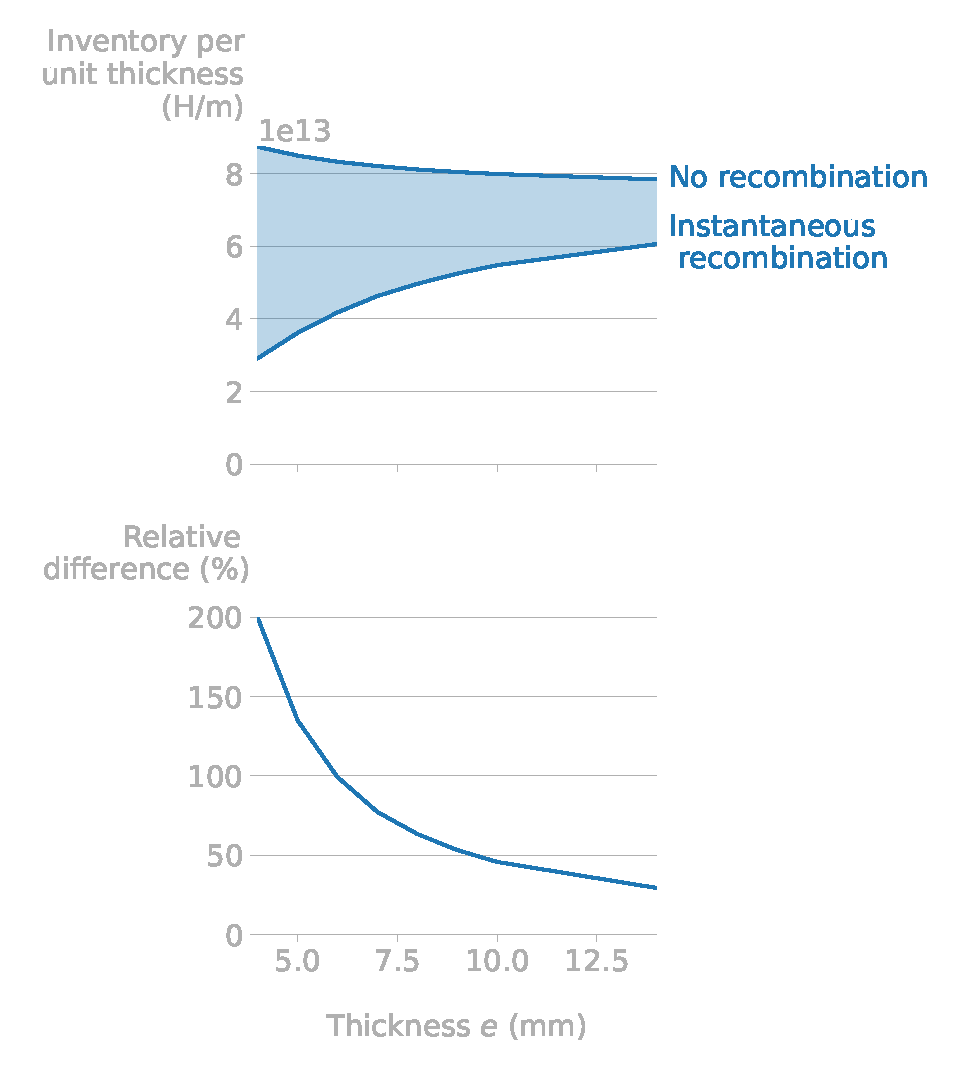
\includegraphics[width=\linewidth]{Figures/Chapter3/monoblocks/3D_monoblocks/inventory_vs_thickness.pdf}
    \caption{Evolution of the inventory with or without recombination at the poloidal gap for several monoblock thicknesses at $t=\SI{1e6}{s}$}
    \label{fig: ratio 3D thickness monoblock}
\end{figure}

% flux
The permeation flux towards the cooling channel per unit thickness globally increases with the monoblock thickness (see Figure \ref{fig: flux to coolant DEMO monoblock}).
It is always higher in the case without recombination on the gaps.
Similarly to the inventory, the relative difference between the cases with or without recombination on the poloidal gap decreases with the thickness.

\begin{figure} [h]
    \centering
    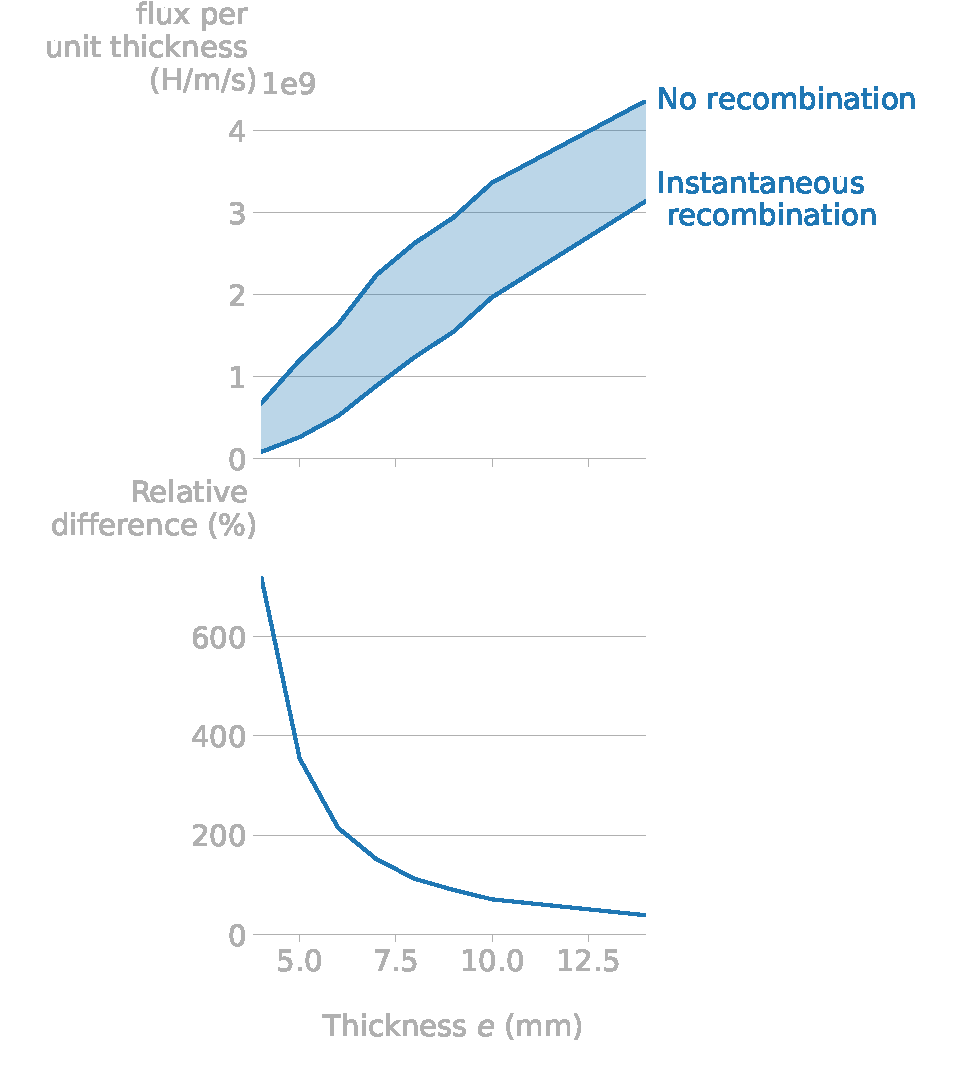
\includegraphics[width=\linewidth]{Figures/Chapter3/monoblocks/3D_monoblocks/permeation_flux_vs_thickness.pdf}
    \caption{Evolution of the permeation flux to the coolant with or without recombination at the poloidal gap for several monoblock thicknesses at $t=\SI{1e6}{s}$.}
    \label{fig: flux to coolant DEMO monoblock}
\end{figure}

% impact of the extrusion
Finally, the extrusion of the CuCrZr pipe between monoblocks has an impact on the permeation flux and the inventory.
Without this extrusion, the case without recombination on the poloidal gap corresponds to a pure 2D case and the inventory is independent of the thickness (see Figure \ref{fig: inventory monoblock vs thickness no gap}).

\begin{figure} [h]
    \centering
    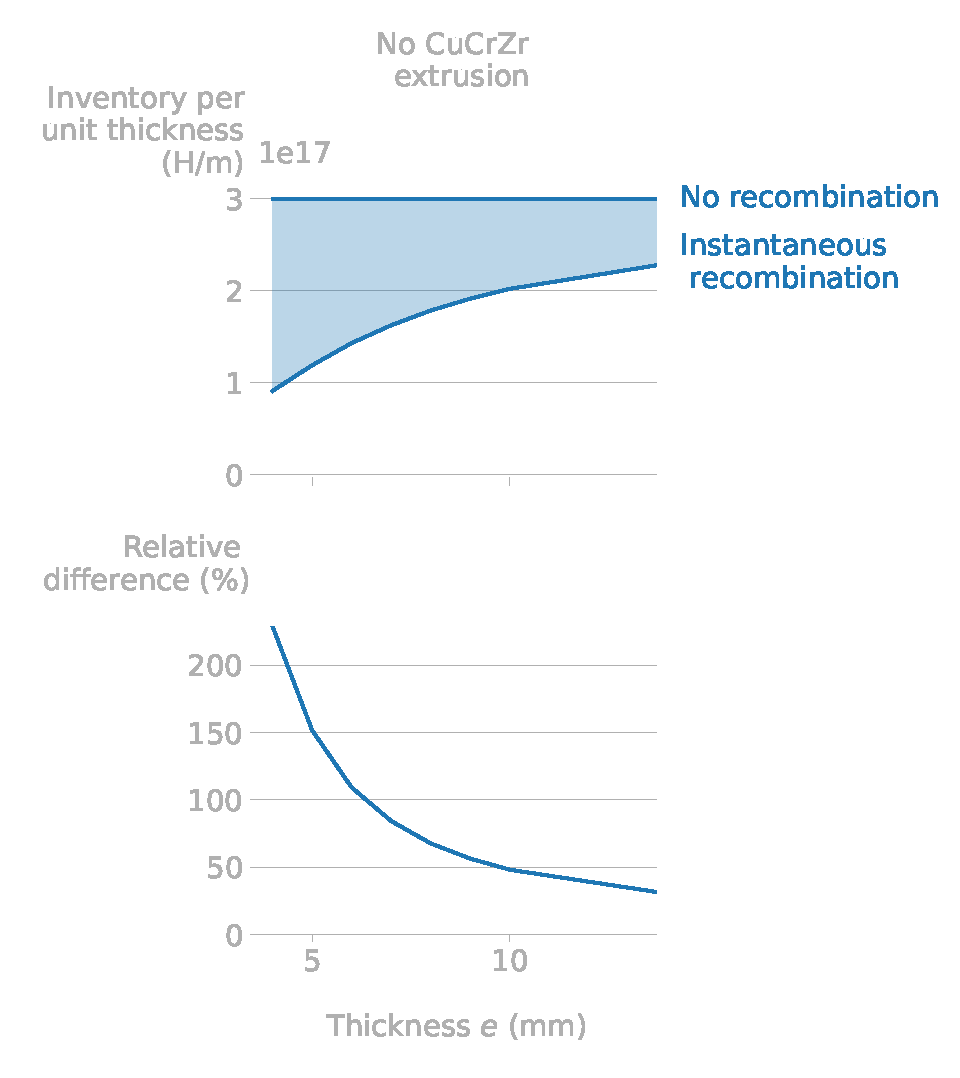
\includegraphics[width=\linewidth]{Figures/Chapter3/monoblocks/3D_monoblocks/inventory_vs_thickness_no_gap.pdf}
    \caption{Evolution of the permeation flux with or without recombination at the poloidal gap for several monoblock thicknesses without CuCrZr extrusion at $t=\SI{1e6}{s}$.}
    \label{fig: inventory monoblock vs thickness no gap}
\end{figure}

\subsection{Summary}
The influence of H desorption on poloidal and toroidal gaps between monoblocks was investigated.
The DEMO baseline geometry (based on an ITER-like concept) was simulated with FESTIM.
It was shown that taking into account recombination on these gaps could drastically decrease the monoblock H inventory (by several orders of magnitude).
In other words, this makes the 2D assumption for monoblocks less valid for (1) thin monoblocks (2) long exposure times.
Indeed, a 2D assumption implies assuming an infinitely thick monoblock (which is totally unrealistic for the ITER and DEMO designs).
However, this assumption is conservative since it will overestimate the H inventory and the permeation flux to the coolant.
Moreover, performing 3D simulations is more computationaly expensive than 2D simulations.
